\begin{figure*}
	\begin{center}
	  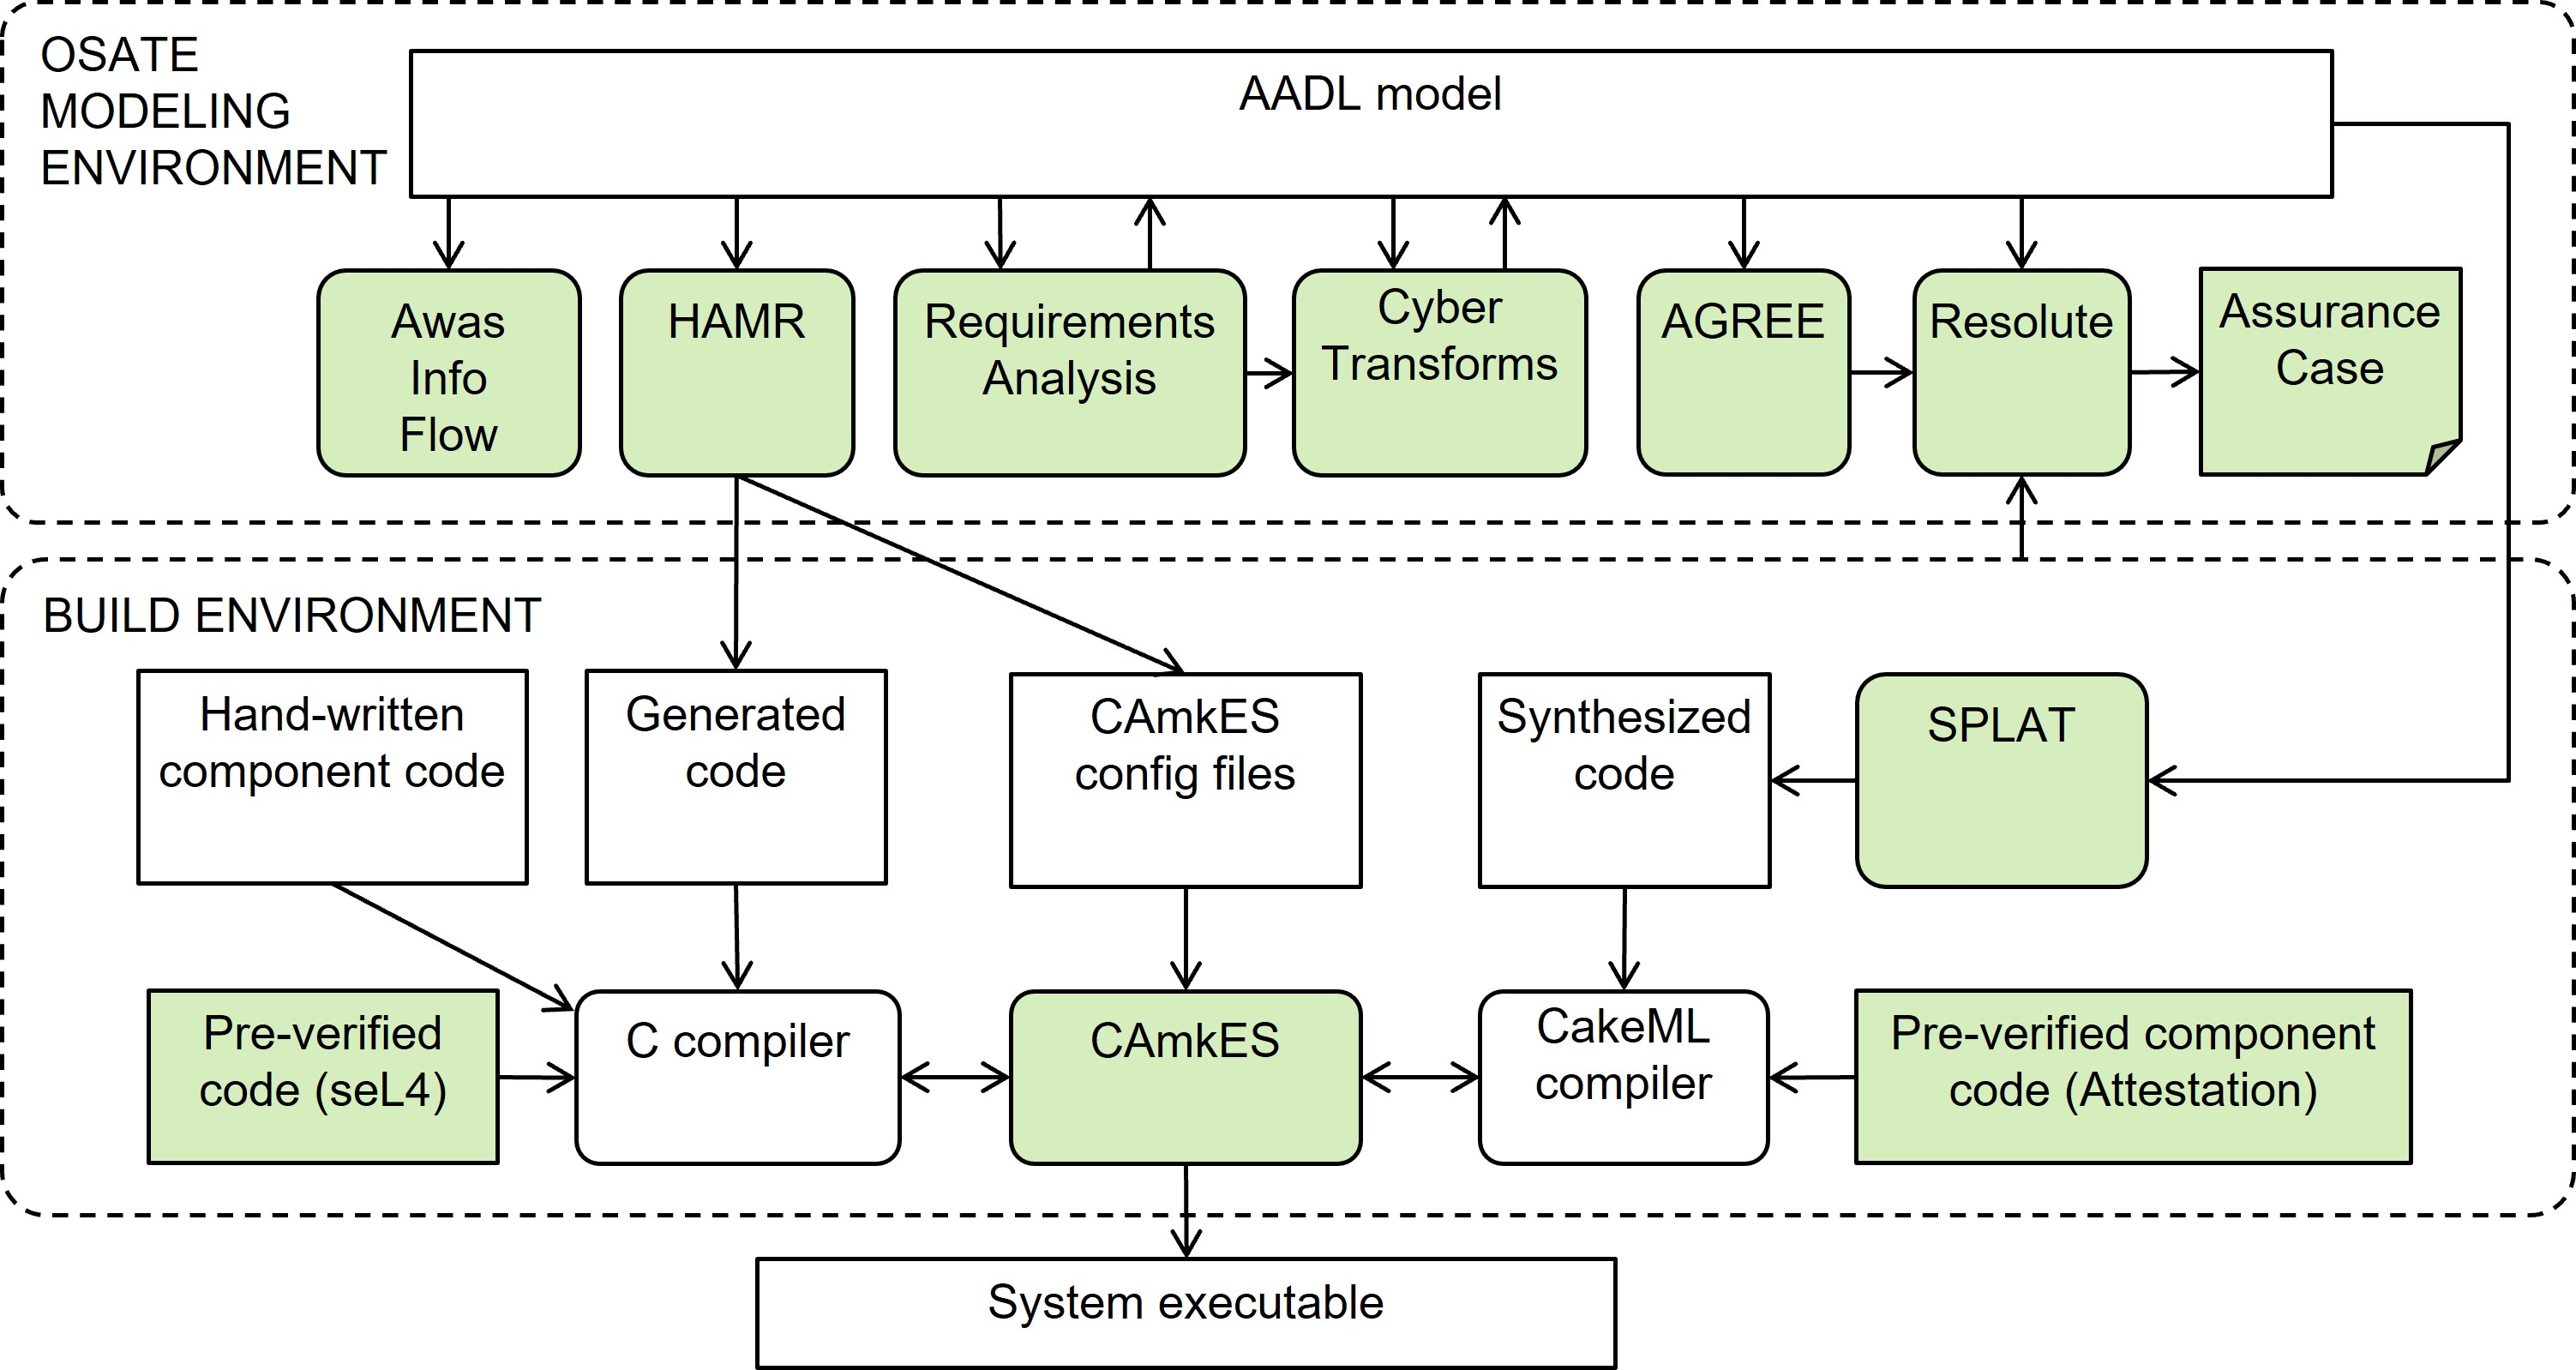
\includegraphics[width=\textwidth]{./figs/tool-arch.jpg}
  	\end{center}
	\caption{\brfcs\ integrated tool architecture with key components in the general workflow shown in green.}
	\label{fig:tool-arch}
\end{figure*}

The \brfcs\ OSATE environment, \figref{fig:tool-arch}, provides
designers with workflow and tool support for developing products with
inherent cyber-resiliency.  It starts with the development of a
baseline AADL model of the system architecture that defines the
desired functionality.  This model can be evaluated on aspects such as
resource usage, information flow, latency analysis, {\etc} using
existing tools.

\brfcs\ integrates additional tools into OSATE to analyze, identify,
and address cybersecurity vulnerabilities in the baseline model (top
of \figref{fig:tool-arch}).  \brfcs\ provides access to analysis tools
that examine the model, report potential cyber vulnerabilities, and
suggest requirements for mitigation \cite{dcrypps2019,gearcase2020}.
Designers add these requirements to the \brfcs\ project requirements
repository.  A key part of the requirements management in \brfcs\ is a
corresponding assurance case that provides evidence, computed directly
from the model or by supporting analysis tools, showing how each
requirement is satisfied.  Evidential statements must exist to address
the added cyber requirements in order for \brfcs\ to build the
assurance case for the project \cite{resolute-destion}.

\brfcs\ provides an extendable library of model transformations to address requirements for common cyber vulnerabilities:
\begin{compactitem}
	\item \textbf{Filter}: block messages that do not conform to a given specification
	\item \textbf{Monitor}: detect and alert violations at runtime
	\item \textbf{Gate}: block messages in the presence of an alert
	\item \textbf{Attestation}: measure non-local software to assess trustworthiness \cite{attestation-copland}
	\item \textbf{Virtualization}: isolate components
	\item \textbf{Proxy}: enable HTTPS message inspection
	\item \textbf{seL4}: transform component definitions for the seL4 secure micro kernel
\end{compactitem}
Transformations update the model's architecture with new components and the assurance case with new required evidential statements.

Filters, monitors, and gates are considered high assurance components that require formal reasoning in building the assurance case.
When added to a system, \brfcs\ requires evidence that such components are
\begin{compactenum}
	\item connected in the model,
	\item cannot be bypassed,
	\item meet their intended purposes, and
	\item are properly implemented.
\end{compactenum}
Information flow analysis provides evidence for the first two properties while model checking and code synthesis provide evidence for the last two properties.

The Awas AADL information flow analyzer and visualizer provides evidence that high assurance components are connected and not bypassed in the model \cite{awas}.
The High Assurance Modeling and Rapid engineering for embedded systems tool (HAMR) generates from the model the infrastructure and integration code that implements the semantics of AADL-compliant scheduling, dispatching, and port-based communication \cite{hamr}.
HAMR additionally constructs a proof that all flows in the model are in the implementation and that no extraneous flows have been added.
HAMR relies on properties of the seL4 microkernel for some aspects of these proofs.
The seL4 microkernel, among other things, provides strong isolation between components ensuring that there are no communication channels outside of what is defined \cite{sel4-sosp09, sel4-tocs14, sel4-cacm18}.

As mentioned earlier,
\agr\ \cite{compositional-analysis-agree,nfm:agree} provides the
formal platform for our work. It bundles together a formal contract
language with a compositional, assume-guarantee-style, model checker
for AADL models.  \agr\ attempts to prove properties about one layer
of the model using properties allocated to sub-components.  The
composition is performed in terms of \emph{contracts} provided for
each component and sub-component that state \emph{assumptions} on
inputs and \emph{guarantees} on outputs under the assumptions.
\agr\ verifies the \emph{consistency} of the composition of the
component and sub-component contracts meaning that in every connection
the source constraints satisfy the destination constraints.

The contributions of this paper relate to the aspects of
\brfcs\ concerning evidence that a high-assurance component meets its
intended purpose and is properly implemented.  This paper defines a
\emph{code contract} language that is a subset of the \agr\ language
with sequential evaluation semantics as opposed to the existing
parallel semantics of \agr.  The sequential semantics are requisite to
code synthesis and are defined such that \agr\ is able to still prove
consistency in the contract composition of the model.

This paper further defines a notion of \emph{test contract} for unit
testing code contracts outside of the system composition to verify
input to output behavior as well as general properties of the code
contract.  In practice, the behavior of a high assurance component is
defined by the designer in a code contract, and then using the
existing \agr\ model checker, test contracts prove the desired code
contract behavior.  Once the designer is satisfied that the code
contract is correct, the system composition is verified to conclude
that the contract meets the original cyber-requirement.

Showing that a component is properly implemented is accomplished
through formal synthesis from the code contract (bottom of
\figref{fig:tool-arch}).  This paper presents the Semantic Properties
of Language and Automata Theory (\splt) tool that generates
\emph{\ckml} code to implement the code contract.  \ckml\ is a
functional language that includes additional proofs and tools built
around it \cite{cakeml}.  The \ckml\ compiler itself is verified to
generate binary implementations that are equivalent in semantics to
the original input program.  That proof ensures that the resulting
binary exactly preserves the meaning of the original code contract and
assures that the component is faithfully implemented.
